\documentclass[portrait,a0paper,fontscale=0.277]{baposter}

\usepackage{calc}
\usepackage{graphicx}
\usepackage{amsmath}
\usepackage{amssymb}
\usepackage{relsize}
\usepackage{multirow}
\usepackage{rotating}
\usepackage{bm}
\usepackage{url}
\usepackage{txfonts}

%\usepackage{wrapfig}

\usepackage{graphicx}
\usepackage{multicol}

%\usepackage{times}
%\usepackage{helvet}
%\usepackage{bookman}
\usepackage{palatino}

\newcommand{\captionfont}{\footnotesize}

\graphicspath{{images/}{../images/}}
\usetikzlibrary{calc}

\newcommand{\SET}[1]  {\ensuremath{\mathcal{#1}}}
\newcommand{\MAT}[1]  {\ensuremath{\boldsymbol{#1}}}
\newcommand{\VEC}[1]  {\ensuremath{\boldsymbol{#1}}}
\newcommand{\Video}{\SET{V}}
\newcommand{\video}{\VEC{f}}
\newcommand{\track}{x}
\newcommand{\Track}{\SET T}
\newcommand{\LMs}{\SET L}
\newcommand{\lm}{l}
\newcommand{\PosE}{\SET P}
\newcommand{\posE}{\VEC p}
\newcommand{\negE}{\VEC n}
\newcommand{\NegE}{\SET N}
\newcommand{\Occluded}{\SET O}
\newcommand{\occluded}{o}


% New definition of square root:
% it renames \sqrt as \oldsqrt
\let\oldsqrt\sqrt
% it defines the new \sqrt in terms of the old one
\def\sqrt{\mathpalette\DHLhksqrt}
\def\DHLhksqrt#1#2{%
\setbox0=\hbox{$#1\oldsqrt{#2\,}$}\dimen0=\ht0
\advance\dimen0-0.2\ht0
\setbox2=\hbox{\vrule height\ht0 depth -\dimen0}%
{\box0\lower0.4pt\box2}}

%%%%%%%%%%%%%%%%%%%%%%%%%%%%%%%%%%%%%%%%%%%%%%%%%%%%%%%%%%%%%%%%%%%%%%%%%%%%%%%%
%%%% Some math symbols used in the text
%%%%%%%%%%%%%%%%%%%%%%%%%%%%%%%%%%%%%%%%%%%%%%%%%%%%%%%%%%%%%%%%%%%%%%%%%%%%%%%%

%%%%%%%%%%%%%%%%%%%%%%%%%%%%%%%%%%%%%%%%%%%%%%%%%%%%%%%%%%%%%%%%%%%%%%%%%%%%%%%%
% Multicol Settings
%%%%%%%%%%%%%%%%%%%%%%%%%%%%%%%%%%%%%%%%%%%%%%%%%%%%%%%%%%%%%%%%%%%%%%%%%%%%%%%%
\setlength{\columnsep}{1.5em}
\setlength{\columnseprule}{0mm}

%%%%%%%%%%%%%%%%%%%%%%%%%%%%%%%%%%%%%%%%%%%%%%%%%%%%%%%%%%%%%%%%%%%%%%%%%%%%%%%%
% Save space in lists. Use this after the opening of the list
%%%%%%%%%%%%%%%%%%%%%%%%%%%%%%%%%%%%%%%%%%%%%%%%%%%%%%%%%%%%%%%%%%%%%%%%%%%%%%%%
\newcommand{\compresslist}{%
\setlength{\itemsep}{1pt}%
\setlength{\parskip}{0pt}%
\setlength{\parsep}{0pt}%
}

%%%%%%%%%%%%%%%%%%%%%%%%%%%%%%%%%%%%%%%%%%%%%%%%%%%%%%%%%%%%%%%%%%%%%%%%%%%%%%
%%% Begin of Document
%%%%%%%%%%%%%%%%%%%%%%%%%%%%%%%%%%%%%%%%%%%%%%%%%%%%%%%%%%%%%%%%%%%%%%%%%%%%%%

\begin{document}

%%%%%%%%%%%%%%%%%%%%%%%%%%%%%%%%%%%%%%%%%%%%%%%%%%%%%%%%%%%%%%%%%%%%%%%%%%%%%%
%%% Here starts the poster
%%%---------------------------------------------------------------------------
%%% Format it to your taste with the options
%%%%%%%%%%%%%%%%%%%%%%%%%%%%%%%%%%%%%%%%%%%%%%%%%%%%%%%%%%%%%%%%%%%%%%%%%%%%%%
% Define some colors

%\definecolor{lightblue}{cmyk}{0.83,0.24,0,0.12}
\definecolor{lightblue}{rgb}{0.145,0.6666,1}

% Draw a video
\newlength{\FSZ}
\newcommand{\drawvideo}[3]{% [0 0.25 0.5 0.75 1 1.25 1.5]
   \noindent\pgfmathsetlength{\FSZ}{\linewidth/#2}
   \begin{tikzpicture}[outer sep=0pt,inner sep=0pt,x=\FSZ,y=\FSZ]
   \draw[color=lightblue!50!black] (0,0) node[outer sep=0pt,inner sep=0pt,text width=\linewidth,minimum height=0] (video) {\noindent#3};
   \path [fill=lightblue!50!black,line width=0pt] 
     (video.north west) rectangle ([yshift=\FSZ] video.north east) 
    \foreach \x in {1,2,...,#2} {
      {[rounded corners=0.6] ($(video.north west)+(-0.7,0.8)+(\x,0)$) rectangle +(0.4,-0.6)}
    }
;
   \path [fill=lightblue!50!black,line width=0pt] 
     ([yshift=-1\FSZ] video.south west) rectangle (video.south east) 
    \foreach \x in {1,2,...,#2} {
      {[rounded corners=0.6] ($(video.south west)+(-0.7,-0.2)+(\x,0)$) rectangle +(0.4,-0.6)}
    }
;
   \foreach \x in {1,...,#1} {
     \draw[color=lightblue!50!black] ([xshift=\x\linewidth/#1] video.north west) -- ([xshift=\x\linewidth/#1] video.south west);
   }
   \foreach \x in {0,#1} {
     \draw[color=lightblue!50!black] ([xshift=\x\linewidth/#1,yshift=1\FSZ] video.north west) -- ([xshift=\x\linewidth/#1,yshift=-1\FSZ] video.south west);
   }
   \end{tikzpicture}
}

\hyphenation{resolution occlusions}
%%
\begin{poster}%
  % Poster Options
  {
  % Show grid to help with alignment
  grid=false,
  % Column spacing
  colspacing=1em,
  % Color style
  bgColorOne=white,
  bgColorTwo=white,
  borderColor=lightblue,
  headerColorOne=black,
  headerColorTwo=lightblue,
  headerFontColor=white,
  boxColorOne=white,
  boxColorTwo=lightblue,
  % Format of textbox
  textborder=roundedleft,
  % Format of text header
  eyecatcher=true,
  headerborder=closed,
  headerheight=0.14\textheight,
%  textfont=\sc, An example of changing the text font
  headershape=roundedright,
  headershade=shadelr,
  headerfont=\normalsize\bf\textsc, %Sans Serif
  textfont={\setlength{\parindent}{1.5em}},
  boxshade=plain,
%  background=shade-tb,
  background=plain,
  linewidth=2pt
  }
  % Eye Catcher
  {
\includegraphics[height=3.25em]{images/logo1-2.jpeg}} 
  % Title
  {\bf\Large{Head-on collisions of Xe atoms against superfluid $^4$He nanodroplets}\vspace{0.5em}}
  % Authors
  {\normalsize{ \underline{F. Coppens}$^1$, A. Leal$^2$, M. Barranco$^{1,2}$, N. Halberstadt$^1$, M. Pi$^2$\vspace{0.5em}} \\
\smaller{$^1$Universit\'e Toulouse 3 and CNRS, Laboratoire des Collisions, Agr\'egats, R\'eactivit\'e, IRSAMC, UMR 5589, 118 route de Narbonne, F-31062 Toulouse Cedex 09, France 
\\ \vspace{2px}
$^2$Departament FQA, Facultat de F\'{\i}sica, and IN$^2$UB, Universitat de Barcelona. Diagonal 645, 08028 Barcelona, Spain

}}
  % University logo
  {% The makebox allows the title to flow into the logo, this is a hack because of the L shaped logo.
   
\includegraphics[height=3.25em]{images/logo_irsamc}
  }

%\vspace{-20px}
\vspace*{0px}
%%%%%%%%%%%%%%%%%%%%%%%%%%%%%%%%%%%%%%%%%%%%%%%%%%%%%%%%%%%%%%%%%%%%%%%%%%%%%%
%%% Now define the boxes that make up the poster
%%%---------------------------------------------------------------------------
%%% Each box has a name and can be placed absolutely or relatively.
%%% The only inconvenience is that you can only specify a relative position 
%%% towards an already declared box. So if you have a box attached to the 
%%% bottom, one to the top and a third one which should be in between, you 
%%% have to specify the top and bottom boxes before you specify the middle 
%%% box.
%%%%%%%%%%%%%%%%%%%%%%%%%%%%%%%%%%%%%%%%%%%%%%%%%%%%%%%%%%%%%%%%%%%%%%%%%%%%%%
    %
    % A coloured circle useful as a bullet with an adjustably strong filling
    \newcommand{\colouredcircle}{%
      \tikz{\useasboundingbox (-0.2em,-0.32em) rectangle(0.2em,0.32em); \draw[draw=black,fill=lightblue,line width=0.03em] (0,0) circle(0.18em);}}

%%%%%%%%%%%%%%%%%%%%%%%%%%%%%%%%%%%%%%%%%%%%%%%%%%%%%%%%%%%%%%%%%%%%%%%%%%%%%%
  \headerbox{Abstract}{name=abstract,column=0,row=0,span=3}{
%%%%%%%%%%%%%%%%%%%%%%%%%%%%%%%%%%%%%%%%%%%%%%%%%%%%%%%%%%%%%%%%%%%%%%%%%%%%%%
%\vspace{2px}  
\scriptsize{
\noindent In the context of dopant dynamics in superfluid helium droplets in vortical states$^1$, we study the head-on collision of a heliophilic xenon atom with a superfluid $^4$He droplet made of  1000  atoms. 
At variance with the findings for a heliophobic cesium atom$^2$ of a similar atomic weight, 
it is found that the xenon atom has to hit the droplet with a large kinetic energy in order to get across it without being captured. 
When it is not captured,  the xenon impurity does not emerge as a bare atom; instead,
due to its heliophilic character it carries away some helium atoms.
}
\vspace{2px}
 }

%%%%%%%%%%%%%%%%%%%%%%%%%%%%%%%%%%%%%%%%%%%%%%%%%%%%%%%%%%%%%%%%%%%%%%%%%%%%%%
  \headerbox{Dynamic evolution}{name=potentials,column=0,row=0,span=1, below=abstract}{
%%%%%%%%%%%%%%%%%%%%%%%%%%%%%%%%%%%%%%%%%%%%%%%%%%%%%%%%%%%%%%%%%%%%%%%%%%%%%%
%\vspace{2px}
\scriptsize{
\noindent Left panel: Xenon atom approaching the $^4$He$_{1000}$ droplet from below at $v_0=200$ m/s. The corresponding time is indicated in each frame. Right panel: Same as left figure for a Cs atom.\\
\vspace{-10px}
\begin{center}  
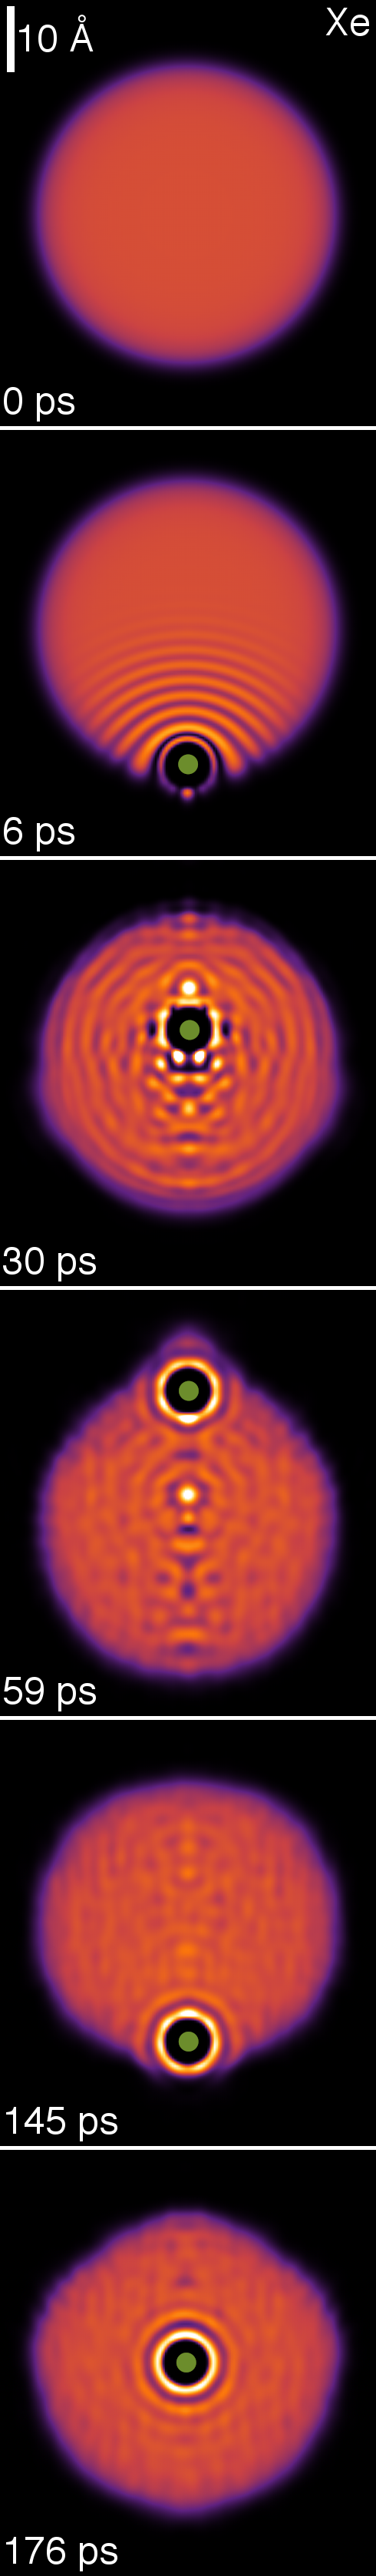
\includegraphics[width=0.410\linewidth]{Xe-vertical}
\hspace{5px}
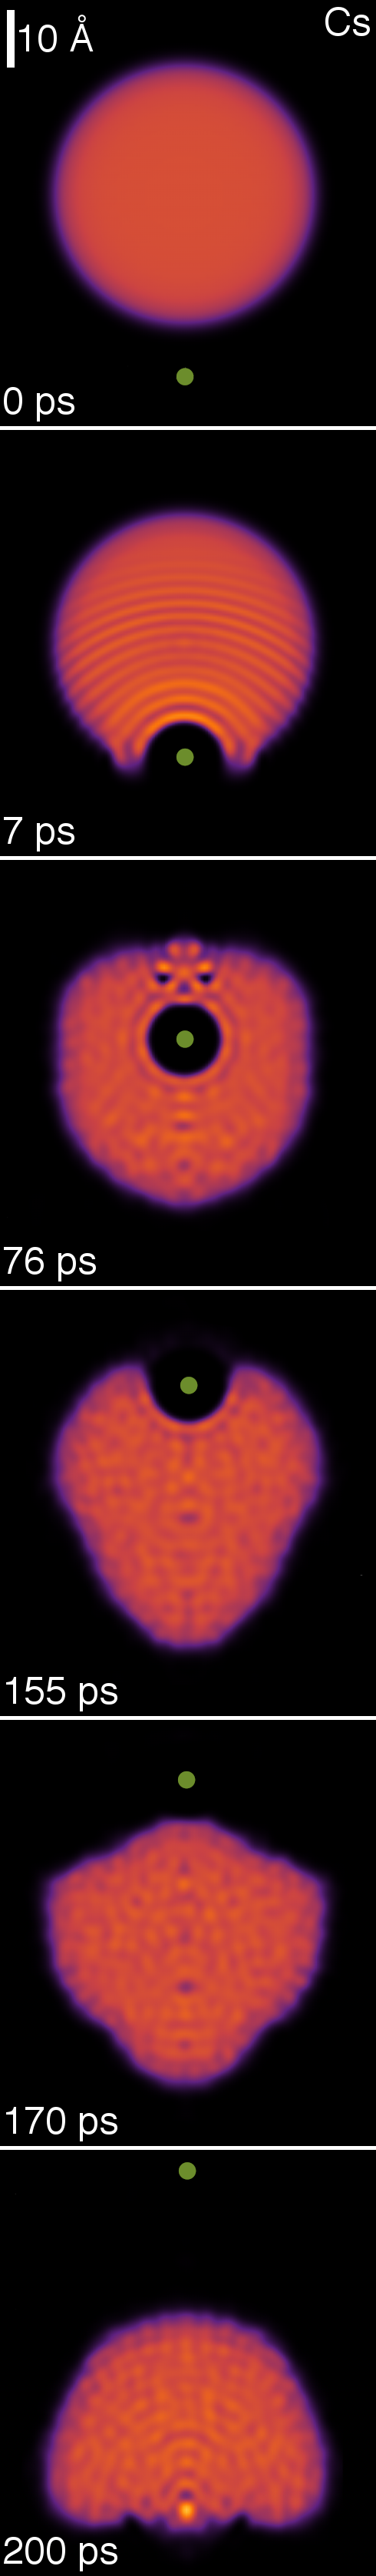
\includegraphics[width=0.410\linewidth]{Cs-vertical}
\end{center}

}
\vspace{2px}
}
 
%%%%%%%%%%%%%%%%%%%%%%%%%%%%%%%%%%%%%%%%%%%%%%%%%%%%%%%%%%%%%%%%%%%%%%%%%%%%%%
  \headerbox{DFT Framework}{name=DFT,column=1,row=0,span=2, below=abstract}{
%%%%%%%%%%%%%%%%%%%%%%%%%%%%%%%%%%%%%%%%%%%%%%%%%%%%%%%%%%%%%%%%%%%%%%%%%%%%%%
\vspace{2px}  
\scriptsize{
\noindent The total energy of the Xe@$^4$He$_{1000}$ complex is based on the density-functional from Ref. [3] and is written as

\begin{align*}
	E[\Psi, \mathbf{r}_{Xe}] = \int d \mathbf{r} \, \frac{\hbar^2}{2m}|\nabla \Psi|^2 + \frac{p^2_{Xe}}{2 m_{Xe}} + \int d \mathbf{r} \, {\cal E}_{He}(\rho)
+ \int d \mathbf{r} \, \rho(\mathbf{r}) \,  V_X(|\mathbf{r}- \mathbf{r}_{Xe}|),
\end{align*}
\noindent where ${\cal E}_{\mathrm{He}}$ is the potential energy per unit volume and $ V_X$ the Xe-He pair potential$^4$.\\
\\
\noindent The following coupled 3D time-dependent system, resulting from the variation of the action, has to be solved to obtain the dynamical evolution. Here the He droplet is represented by a complex effective wave function $\Psi_{\mathrm{He}}(\mathbf{r},t)$; the Xe atom is represented by its classical position  $\mathbf{r}_{\mathrm{Xe}}(t)$ obeying Newton's equation of motion

\begin{align*}
	i\hbar\frac{\partial}{\partial t} \Psi_{\mathrm{He}} &= \left[-\frac{\hbar^2}{2m_{\mathrm{He}}}\nabla^2 + \frac{\delta {\cal E}_{\mathrm{He}}}{\delta \rho(\mathbf{r})} + V_X(|\mathbf{r}- \mathbf{r}_{\mathrm{Xe}}|) \right] \Psi_{\mathrm{He}} \\
	m_{\mathrm{Xe}} \ddot{\mathbf{r}}_{\mathrm{Xe}} &= - \nabla_{\mathbf{r}_{\mathrm{Xe}}} \left[ \int d \mathbf{r} \rho(\mathbf{r}) V_X(|\mathbf{r}- \mathbf{r}_{\mathrm{Xe}}|) \right] = -  \int d \mathbf{r} [\nabla \rho(\mathbf{r})] V_X(|\mathbf{r}- \mathbf{r}_{\mathrm{Xe}}|).
\end{align*}

}
\vspace{-0px}
 }
 
%%%%%%%%%%%%%%%%%%%%%%%%%%%%%%%%%%%%%%%%%%%%%%%%%%%%%%%%%%%%%%%%%%%%%%%%%%%%%%
  \headerbox{Configuration stability}{name=dynamics,column=1,row=0,span=2, below=DFT}{
%%%%%%%%%%%%%%%%%%%%%%%%%%%%%%%%%%%%%%%%%%%%%%%%%%%%%%%%%%%%%%%%%%%%%%%%%%%%%%
\vspace{2px}  
\scriptsize{
\noindent Energy of the Xe@$^4$He$_{1000}$ complex as a function of the
distance between  the Xe atom and the  COM of the droplet.
Several two-dimensional helium densities and density profiles are shown for distances between 0 and 40 \AA{} in 5  \AA{} steps.
Connected (dots) and disconnected (triangles) helium configurations are shown \emph{(see text)}.
Top left inset: Snapshot of the helium density at the
first turning point  during the dynamic evolution of a Xe atom (green dot)  at  $v_0 = 600$ m/s 
attained  78 ps after it has started.

\begin{center}
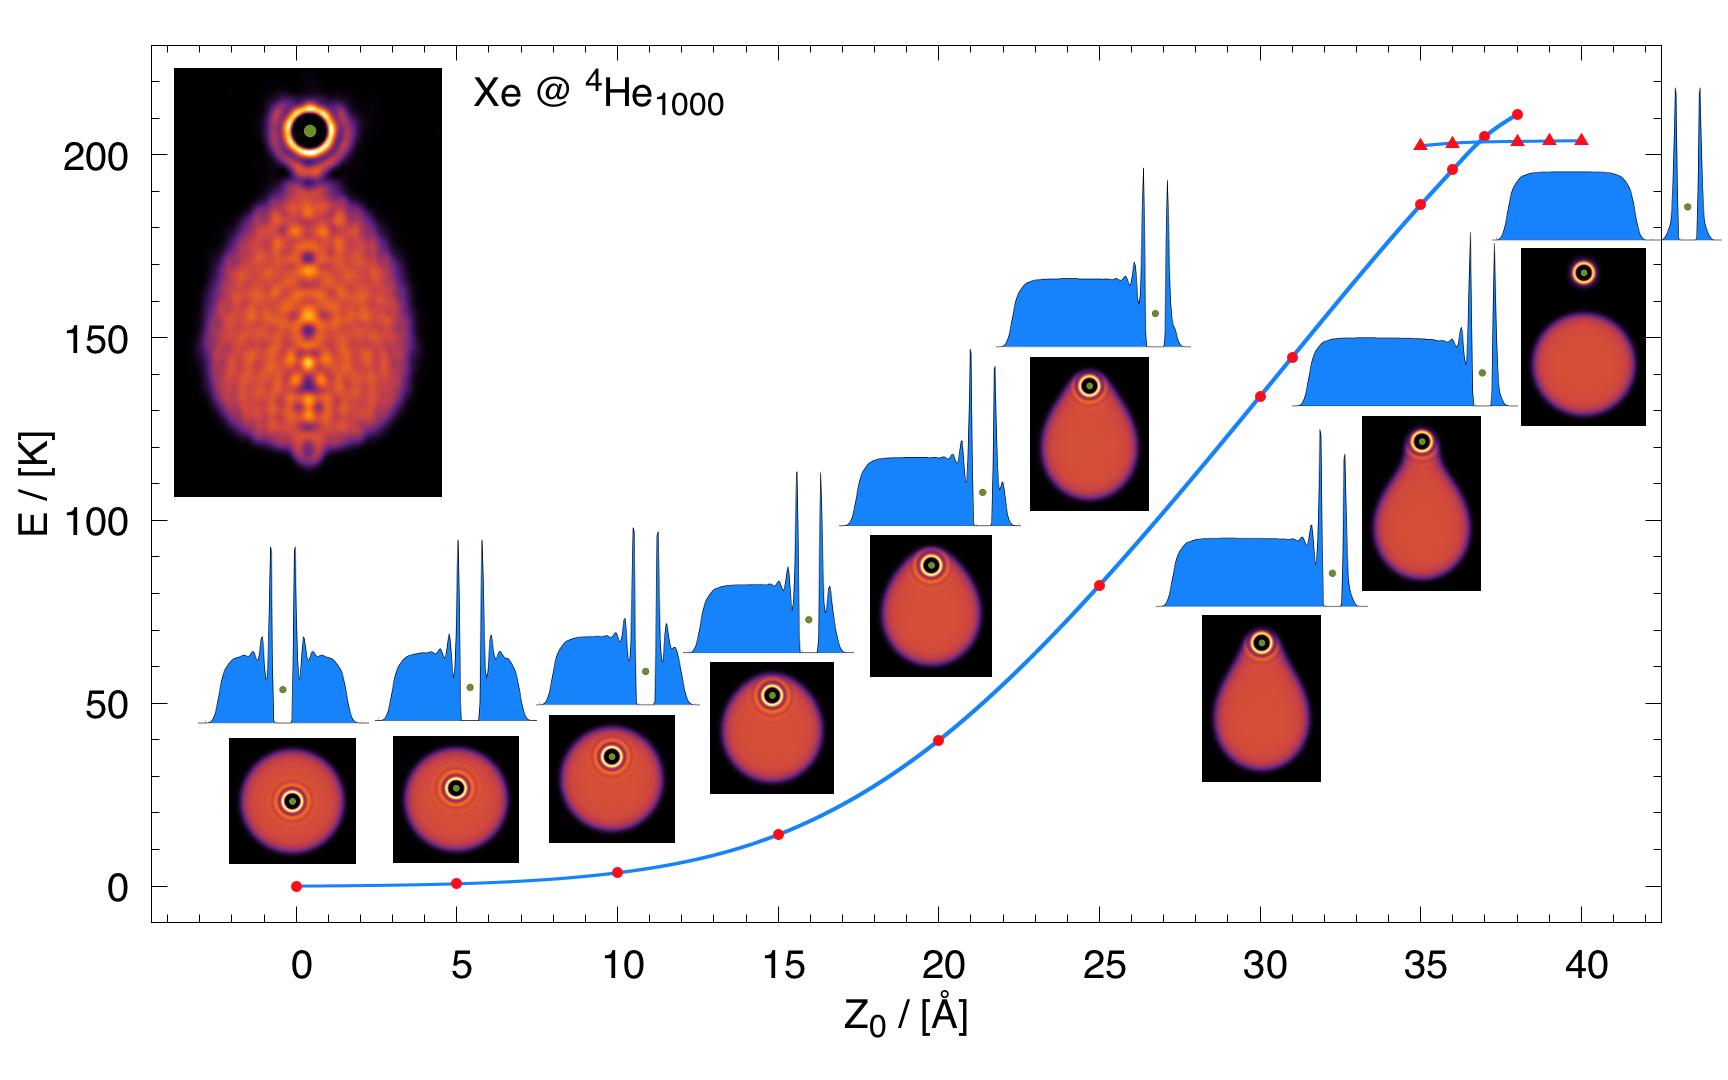
\includegraphics[width=0.82\linewidth]{Xe-4He1000-constraint}\\
\end{center}
}
\vspace{2px}
 }
 
%%%%%%%%%%%%%%%%%%%%%%%%%%%%%%%%%%%%%%%%%%%%%%%%%%%%%%%%%%%%%%%%%%%%%%%%%%%%%%
  \headerbox{Energetics and phase-space}{name=spectra,column=1,span=2, below=dynamics, above=bottom}{
%%%%%%%%%%%%%%%%%%%%%%%%%%%%%%%%%%%%%%%%%%%%%%%%%%%%%%%%%%%%%%%%%%%%%%%%%%%%%%
\vspace{5px}  
\scriptsize{
\noindent Kinetic and total (kinetic plus potential) energy as a function of time of a Xe atom head-on colliding against a $^4$He$_{1000}$ 
droplet at $v_0=200$ m/s (left figure), and the same for a Cs atom (middle figure). The vertical arrows indicate the first two turning points
at 59 and 145 ps.
%\vspace{-5px}
\begin{center}
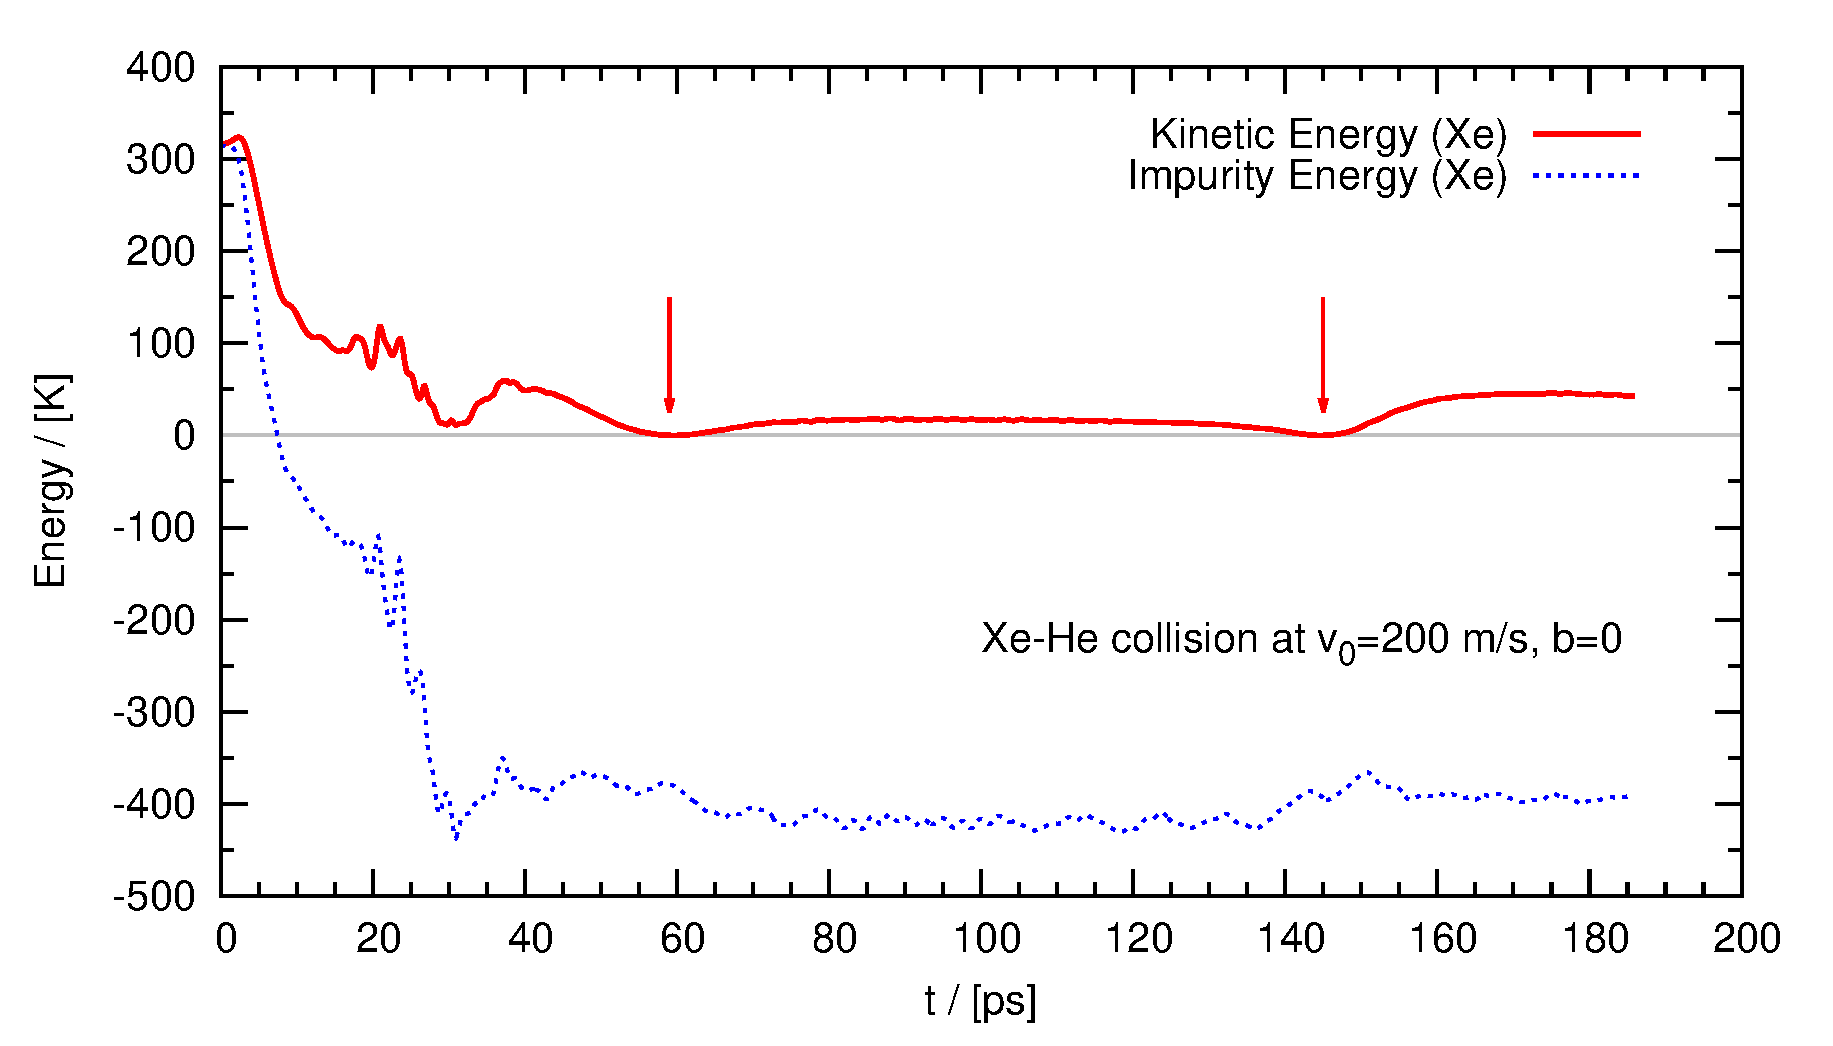
\includegraphics[width=0.33\linewidth]{fig3-Xe-He}
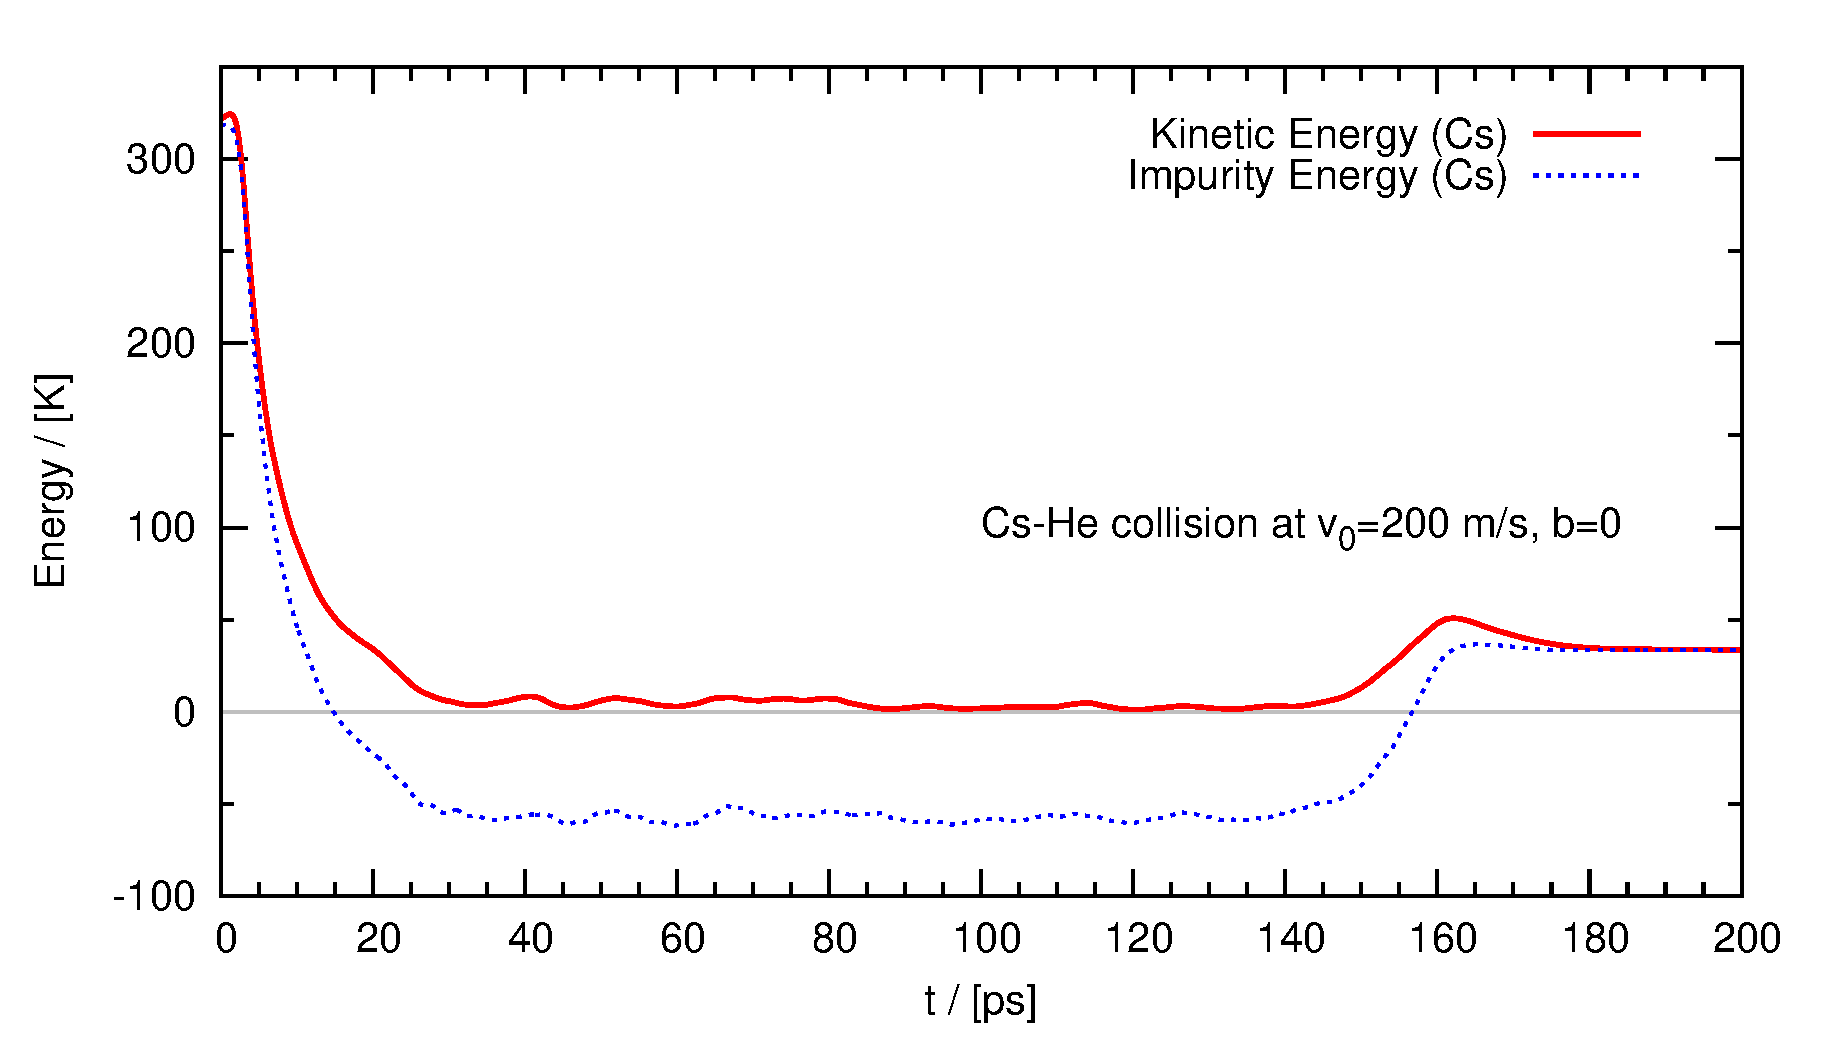
\includegraphics[width=0.33\linewidth]{fig3-Cs-He}
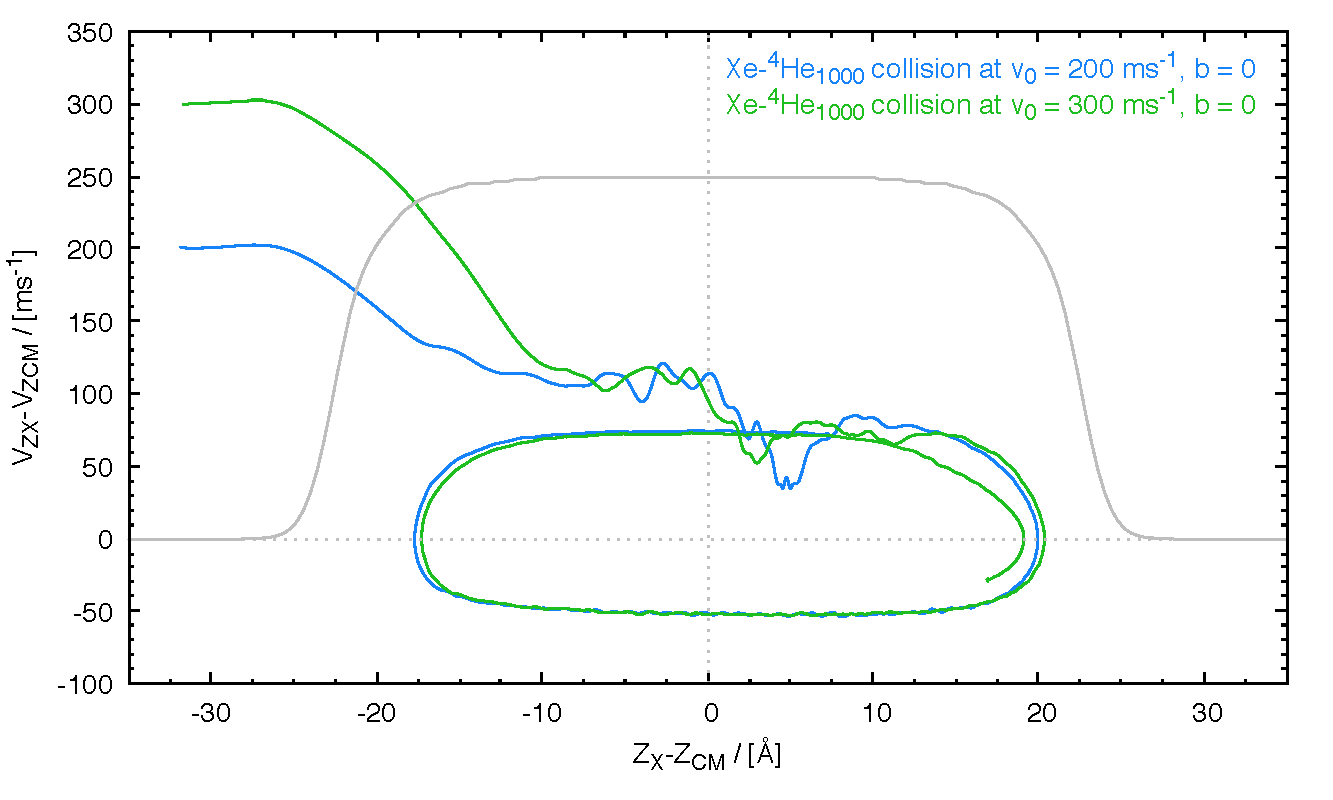
\includegraphics[width=0.33\linewidth]{Phase}
\end{center}
%\vspace{-5px}
\noindent On the right a phase-diagram is shown that demonstrates that the average velocity of the Xe atom in the droplet is lower than the Landau critical velocity, and that it is independent of the initial velocity.

}
\vspace{5px}
 }
 

%%%%%%%%%%%%%%%%%%%%%%%%%%%%%%%%%%%%%%%%%%%%%%%%%%%%%%%%%%%%%%%%%%%%%%%%%%%%%%
  \headerbox{References}{name=references,column=0,span=1, below=potentials, above=bottom}{
%%%%%%%%%%%%%%%%%%%%%%%%%%%%%%%%%%%%%%%%%%%%%%%%%%%%%%%%%%%%%%%%%%%%%%%%%%%%%%
\vspace{2px}  
\scriptsize{ \vspace{2px}
\noindent [1] L.F. Gomez et al., Science \textbf{345}, 906 (2014) \\ 
\noindent [2] A. Leal, D. Mateo, A. Hernando, M. Pi, M. Barranco, Phys. Chem. Chem. Phys. \textbf{16}, 23206 (2014)\\
\noindent [3] F. Ancilotto, M. Barranco, F. Caupin, R. Mayol, M. Pi, Phys. Rev. B  \textbf{72}, 214522 (2005) \\
\noindent [4] K.T. Tang, J.P. Toennies, Z. Phys. D \textbf{1}, 91 (1986)

}

\vspace{2px}
 }
 
\end{poster}

\end{document}

